%---------------------------------------------------------------------------------------------
\subsection{Gastos Legales}

La creación de una sociedad implica una serie de gastos legales necesarios para cumplir con las normativas vigentes y asegurar su correcta constitución. Estos gastos incluyen tarifas administrativas, honorarios profesionales y otros costos relacionados.En la Tabla \ref{tab:costos_legales} se detallan los costos legales asociados a la creación de la sociedad.

\begin{table}[ht]
    \centering
    \caption{Gastos legales de creación de la sociedad.}
    \label{tab:costos_legales}
    \begin{tabularx}{\textwidth}{|X|r|} 
        \hline
        \textbf{Descripción} & \textbf{Costo (Bs)} \\ \hline
        Arancel de Seprec & 455 \\ 
        Publicación Gaceta & 192 \\ 
        Balance de apertura del contador & 200 \\ 
        Gobierno autónomo municipal Santa Cruz & 150 \\ 
        Honorarios notario & 500 \\ 
        Honorarios abogado & 3500 \\ \hline
        \textbf{TOTAL} & \textbf{4997} \\ \hline
    \end{tabularx}
\end{table}

%---------------------------------------------------------------------------------------------
%---------------------------------------------------------------------------------------------
\section{Evaluación de Proyecto de Inversión}
La evaluación de un proyecto de inversión es fundamental para determinar su viabilidad y potencial de rentabilidad. En esta sección, se abordan tres elementos clave: la comparación costo-beneficio, el Valor Actual Neto (VAN) y la Tasa Interna de Retorno (TIR). Estos indicadores financieros proporcionan una comprensión profunda de los ingresos proyectados frente a los costos, la rentabilidad esperada descontada a valor presente y la eficiencia general del proyecto. Este análisis integral permite tomar decisiones informadas y estratégicas sobre la inversión.

%---------------------------------------------------------------------------------------------
\subsection{Comparación Costo Beneficio}

El análisis financiero del proyecto asumiendo el modelo de negocio SaaS con la proyección del proyecto completo. Se calculó la relación entre los ingresos y costos anuales asumiendo un programador junior contratado para realizar el desarrollo y mantenimiento continuo del sistema; Ademas que inicialmente que se capta al 10\% del mercado potencial como usuario mismos que incrementan según la tasa de incremento de profesionales SySO anual del $58.8\%$ visible en la Figura \ref{fig:profesionales_syso_registrados}. Los resultados de la proyección se presentan en la Tabla \ref{tab:proyeccion_financiera} en la que se utilizó un un costo por membresía de Bs.70. La relación costo-beneficio mejora significativamente a lo largo de los años, comenzando en 1.00 en el primer año y alcanzando 18 en el quinto año. Esto indica que, para el quinto año, por cada boliviano invertida, se generan alrededor de 18 bolivianos en ingresos.

\begin{table}[htb]
    \caption{Proyección financiera del proyecto bajo el modelo SaaS.}
    \label{tab:proyeccion_financiera}
    \centering
    \begin{tabularx}{\textwidth}{|l|r|>{\raggedleft\arraybackslash}X|>{\raggedleft\arraybackslash}X|>{\raggedleft\arraybackslash}X|r|}
        \hline
        \thead{Año} & \thead{Usuarios\\Mensuales} & \thead{Gastos\\Anuales (Bs)}  & \thead{Ingresos\\Anuales (Bs)}  & \thead{Balance\\Anual (Bs)} & \thead{C/B} \\ \hline
        0 & 0 & 276,755.53 & 00.00 & -276,755.53 & 0.00 \\ \hline
        1 & 330 & 98,688.72 & 277,200.00 & 178,511.28 & 2.81 \\ \hline
        2 & 525 & 98,688.72 & 441,000.00 & 342,311.28 & 4.47 \\ \hline
        3 & 834 & 98,688.72 & 700,560.00 & 601,871.28 & 7.10 \\ \hline
        4 & 1325 & 98,688.72 & 1,113,000.00 & 1,014,311.28 & 11.28 \\ \hline
        5 & 2104 & 98,688.72 & 1,767,360.00 & 1,668,671.28 & 17.91 \\ \hline
    \end{tabularx}
\end{table} 

%---------------------------------------------------------------------------------------------
\subsection{Valor Actual Neto}
El Valor Actual Neto (VAN) es una medida financiera que calcula la diferencia entre el valor presente de los flujos de efectivo entrantes y salientes de un proyecto. Se calcula descontando los flujos de caja futuros a una tasa de descuento y restando la inversión inicial. Para este proyecto, se utiliza una tasa de descuento del 10\%. 

\begin{equation}
    \label{eq:VAN}
    VAN = \sum \frac{ganancias}{(1+K)^{n}} - \sum \frac{costos}{(1+K)^{n}}
\end{equation}

\begin{equation*}
    VAN =  2,135,932.70
\end{equation*}

El VAN se calcula restando los flujos de efectivo descontados de los costos descontados, lo que da como resultado un VAN de 2,464,402.58. Esto indica que, después de descontar los flujos de efectivo futuros y la inversión inicial, el proyecto en cuestión generaría un valor adicional de 2,464,402.58 en términos de valor presente neto. Este resultado sugiere que el proyecto tiene un potencial de rentabilidad positivo y podría ser una inversión atractiva.

%---------------------------------------------------------------------------------------------
\subsection{Tasa Interna de Retorno}
La Tasa Interna de Retorno (TIR) es un indicador financiero utilizado para evaluar la rentabilidad de una inversión. Representa la tasa de descuento que iguala el VAN de una serie de flujos de caja a cero. En otras palabras, la TIR es la tasa de interés que hace que el valor presente de los ingresos futuros de una inversión sea igual al costo inicial de la misma.
\begin{equation}
    \label{eq:TIR}
    VAN = \sum_{t=1}^{n} \frac{F_t}{(1+TIR)^{t-1}} - I = 0
\end{equation}
\indent
En la ecuación \ref{eq:TIR}, $F_t$ son los flujos de caja en el periodo $t$, $n$ es el número total de periodos, e $I$ es la inversión inicial. La misma se resuelve iterativamente, ya que no tiene una solución algebraica directa, especialmente cuando los flujos de caja no son constantes. El valor de la TIR es útil porque permite comparar la rentabilidad de diferentes proyectos de inversión. En general, un proyecto se considera aceptable si su TIR es mayor que la tasa mínima de rendimiento requerida o el costo de oportunidad del capital. En el contexto del proyecto evaluado, se ha determinado que la TIR es del 112\%. Este valor indica una alta rentabilidad del proyecto, ya que la tasa de retorno esperada es significativamente superior al costo de capital típico en muchos sectores.

%---------------------------------------------------------------------------------------------
\subsection{Conclusión}
La evaluación del proyecto de inversión mediante la comparación costo-beneficio, el VAN y el TIR revela una perspectiva prometedora. La proyección financiera muestra una mejora constante en la relación costo-beneficio, culminando en una relación de 18:1 para el quinto año. El VAN positivo de 2,135,932.70 sugiere que el proyecto no solo recuperará la inversión inicial sino que también generará un valor neto significativo. La TIR del 112\% indica una alta rentabilidad, superando ampliamente las tasas de retorno estándar en la industria. Estos resultados combinados apoyan la viabilidad y rentabilidad del proyecto, recomendando su implementación como una inversión estratégica y beneficiosa.

%---------------------------------------------------------------------------------------------
%---------------------------------------------------------------------------------------------
\section{Análisis de Competidores}

Se realizó un análisis de competidores para identificar oportunidades y amenazas en el mercado, así como para comprender la posición relativa del producto propuesto frente a sus rivales, lo cual permite formular estrategias efectivas y diferenciarse en el mercado del software de gestión de salud y seguridad. 

A nivel mundial, el mercado del software de salud y seguridad ocupacional se compone de dos tipos predominantes: soluciones basadas en la nube y soluciones basadas en la web. El software basado en la nube se refiere a un sistema al que se accede a través de internet, donde los datos se almacenan y procesan en servidores remotos. Ofrece mayor flexibilidad, escalabilidad y accesibilidad. Por otro lado, el software basado en la web funciona a través de un navegador web, requiriendo conectividad a internet. Proporciona comodidad y facilidad de uso, ya que los usuarios pueden acceder al software desde cualquier dispositivo con un navegador. Subdividiéndose por aplicación en: `Grandes empresas' y `Pequeñas y Medianas Empresas' (PyME). Las grandes empresas necesitan software que gestione eficazmente la salud y seguridad ocupacional en diversos departamentos y ubicaciones, debido a su estructura compleja y mayor cantidad de empleados. Las PyMEs, en cambio, requieren soluciones rentables que cubran sus necesidades de gestión de salud y seguridad. Por lo tanto, el mercado ofrece aplicaciones de software adaptadas a ambos segmentos para cumplir con sus requisitos específicos y asegurar la conformidad con las normativas de salud y seguridad (\cite{KingpinMarketResearch}).

Rápidamente la Figura~\ref{fig:visitas_por_dominio} permite observar que las tres compañías con mayor ocupación del mercado en lo que a tráfico de red se refiere son \textit{sitedocs}, \textit{donesafe} y \textit{everbridge}. Estas tres empresas juntas representan más del 50\% del tráfico total, destacando su fuerte presencia y dominio en el mercado (\cite{SEMrushMarketExplorer}).

\begin{figure}[htb]
    \centering
    \fbox{
        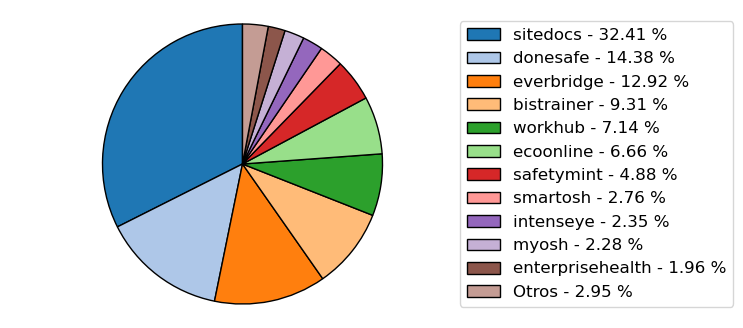
\includegraphics[width=0.95\linewidth]
        {images/marcopractico/planificacion/visitas_por_dominio.png}
    }
    \caption{Participación de Mercado de los Principales Competidores}
    \footnotesize{{Elaboración propia a partir de datos obtenidos por medio de ``\textit{\citefield{SEMrushMarketExplorer}{title}}'' (\citeyear{SEMrushMarketExplorer}).}}
    \label{fig:visitas_por_dominio}
\end{figure}

A su vez, la matriz ilustrada en la Figura~\ref{fig:MatrizCompetidores}, divide los dominios en cuatro categorías: Jugadores de nicho, agentes de cambio, líderes y jugadores establecidos. El eje X representa el volumen total de tráfico que reciben los dominios, mientras que el eje Y muestra el porcentaje de crecimiento del tráfico total. Cada punto en el gráfico representa un dominio y su trayectoria de crecimiento durante el período seleccionado. Las líneas que conectan los puntos iniciales y finales muestran el cambio en el tráfico y la tasa de crecimiento a lo largo del tiempo.

\begin{figure}[htb]
    \centering
    \fbox{
        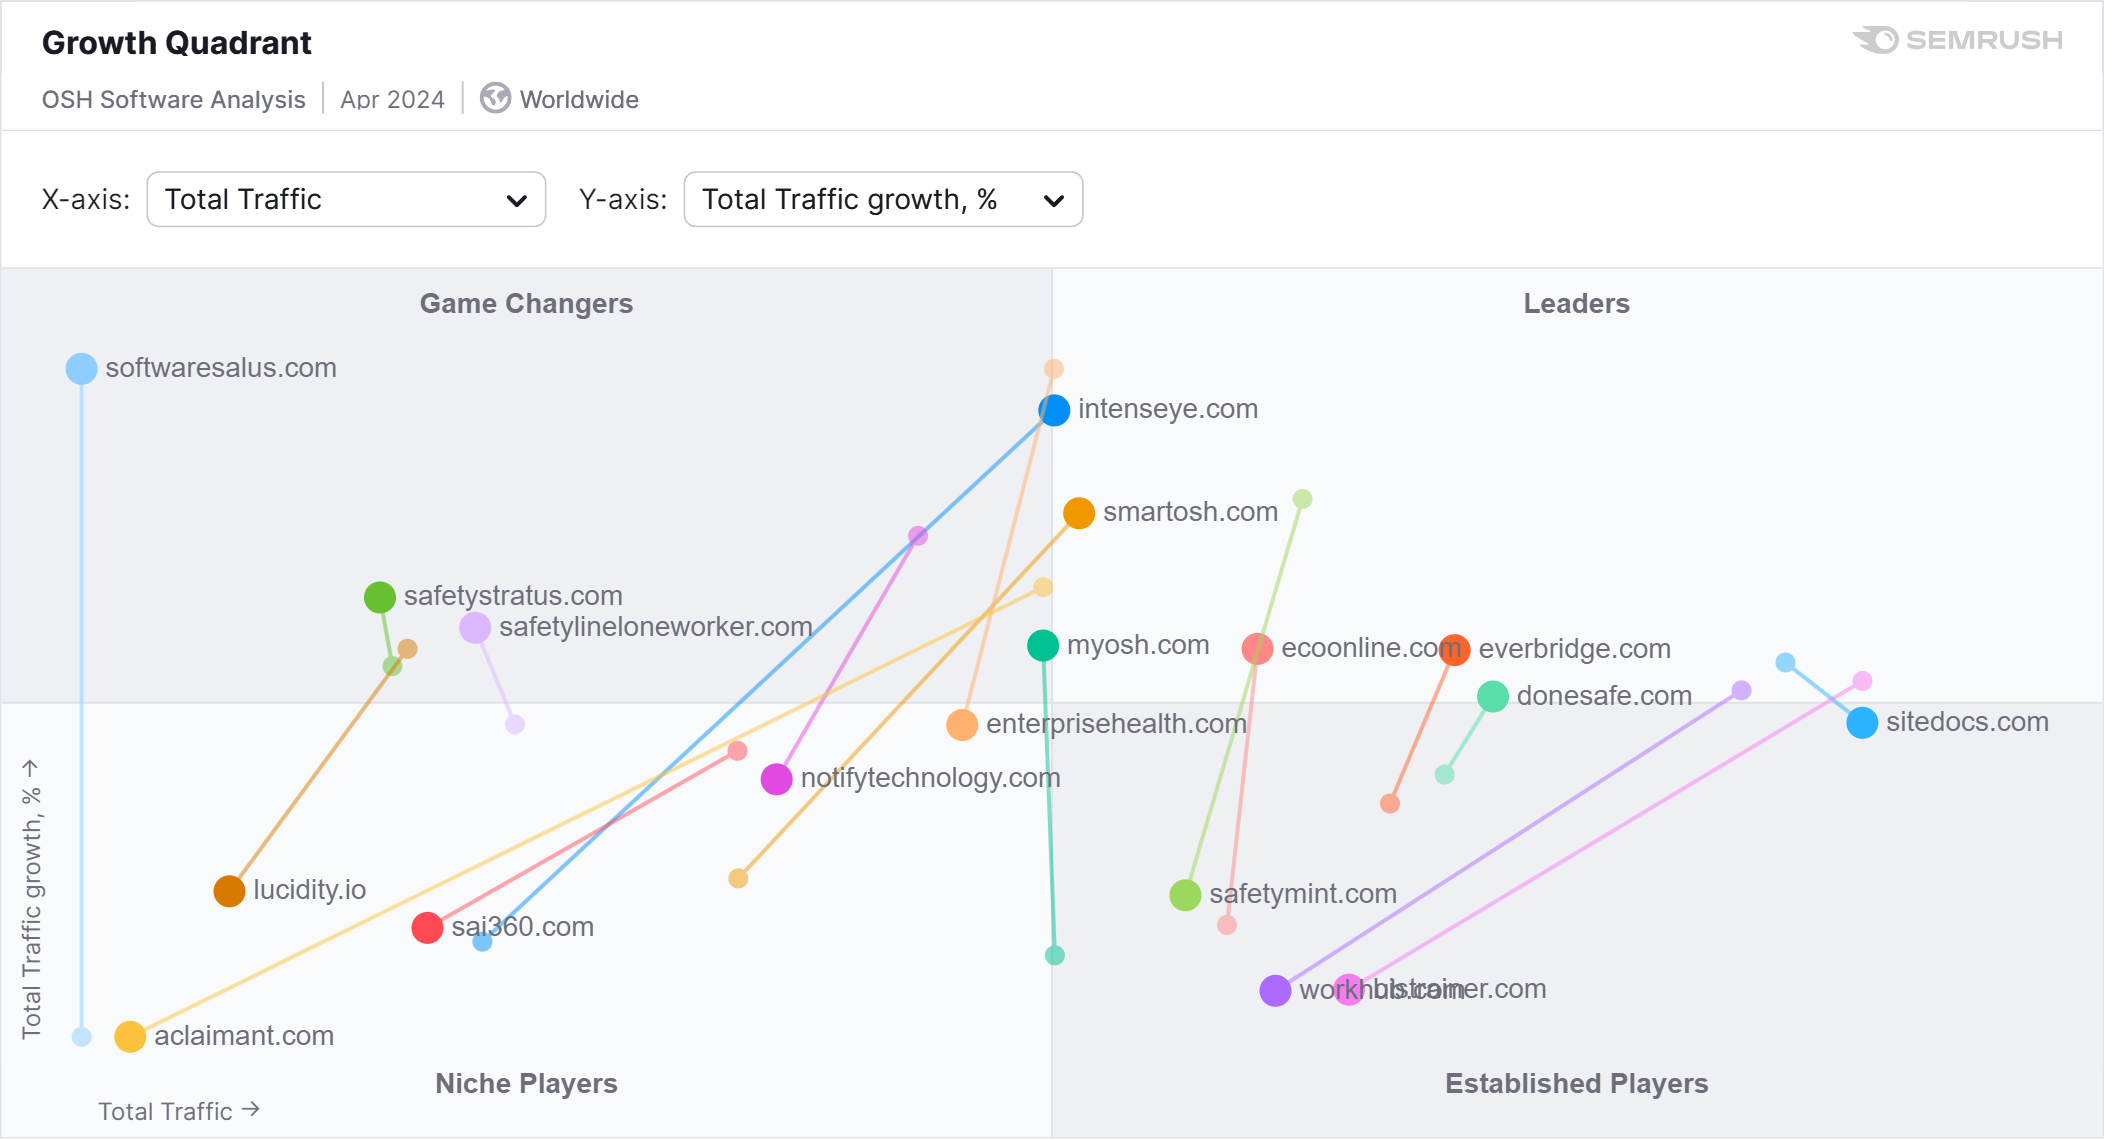
\includegraphics[width=0.95\linewidth]
        {images/marcopractico/planificacion/GrowthQuadrant.png}
    }
    \caption{Matriz de Competidores: \textit{OSH Software}}
	\footnotesize{Fuente: Elaborado por \cite{SEMrushMarketExplorer}.}
    \label{fig:MatrizCompetidores}
\end{figure}

En esta matriz, \textit{sitedocs} se encuentra claramente en la categoría de líderes, no solo por su alto volumen de tráfico, sino también por un crecimiento positivo. Destacan los casos de \textit{intenseye} y \textit{smartosh} que también están en la categoría de líderes, mostrando un crecimiento significativo desde la categoría de jugadores de nicho. Por otro lado, dominios como \textit{softwareasalus} están catalogados como agentes de cambio debido a su impresionante crecimiento en el tráfico, aunque su volumen total de tráfico sea menor. Los jugadores establecidos, como \textit{donesafe} y \textit{workhub}, tienen un alto volumen de tráfico pero un crecimiento más estable y menos pronunciado.\\ \indent
Se puede concluir, en primer lugar que los agentes de cambio, como \textit{softwareasalus}, aunque tienen menor volumen de tráfico, están creciendo rápidamente, lo que sugiere que nuevas empresas pueden irrumpir en el mercado con innovaciones significativas y atraer rápidamente a los usuarios. Además, los jugadores establecidos, con su tráfico consolidado pero crecimiento lento, representan una estabilidad en el mercado, ofreciendo una base de comparación para el rendimiento y las estrategias de retención de usuarios.

